\documentclass[a4paper]{article}
\usepackage[a4paper, total={17cm, 25.7cm}]{geometry}
\usepackage[main=english]{babel} % lingua 
\fontsize{12}{12}

\usepackage{graphicx, physics, hyperref, tikz}
\usepackage{subcaption}
\usepackage{wrapfig}
\usepackage{amsmath}
\usepackage{amssymb}
\usepackage{float}
\usepackage{hyperref}
\usepackage{siunitx}

\usepackage[style=ieee]{biblatex}
\addbibresource{biblio.bib}

\setlength{\parindent}{0pt}


\title{Simulation using MEEP library}
\author{Elisabetta Ferri}
\date{\today}

\begin{document}

\maketitle
 
\begin{abstract}

The results produced by the simulation of photonics elements are presented. Using the MEEP software, three elements were simulated: a directional coupler, a Bragg rifractor and a micro ring resonator. The simulations are available on the Git repository\cite{Git_repo}.

\end{abstract}

\section{Introduction}
Meep is a free and open-source software package for the simulation of electromagnetic fields via the finite-difference time-domain (FDTD) method.
Its application extends also to the simulation of photonic elements and circuits.  

The FDTD method is a widely used technique: the space is divided into a discrete grid and the fields are evolved in discrete time steps.
The discretization of time is directly determined by the space discretization and as the steps are made finer and finer, the simulation becomes a closer and closer approximation for the true continuous equations.

Considering the 1D case for simplicity, the FDTD algorithm starts from Faraday's and Ampere's laws written in Eq. \ref*{eq:Faraday_Ampere}.
\begin{equation} \label{eq:Faraday_Ampere}
    \mu \pdv{H_y}{t} = \pdv{E_z}{x} \qquad\qquad\qquad \varepsilon \pdv{E_z}{t} = \pdv{H_y}{x}
\end{equation}
As the space and time are discretized, the electric and magnetic fields can be written using a discrete notation as \(E_z(x, t) = E_z (m\Delta x, q \Delta t) = E_z^q[m]\) and \(H_y(x, t) = H_y(m\Delta x, q \Delta t) = H_y^q[m]\). This allows to replace the derivatives in the laws with finite differences, obtaining the difference equation in Eq.s \ref*{eq:difference_eqs_E} and \ref*{eq:difference_eqs_B}.
\begin{align}
    \label{eq:difference_eqs_E}
    \mu \frac{H_y^{q+\frac{1}{2}}[m+\frac{1}{2}] - H_y^{q-\frac{1}{2}}[m+\frac{1}{2}]}{\Delta t} = \frac{E_z^q[m+1] - E_z^q[m]}{\Delta x}
    \\
    \label{eq:difference_eqs_B}
    \varepsilon\frac{E_z^{q+1}[m] - E_z^q[m]}{\Delta t} = \frac{H_y^{q+\frac{1}{2}}[m+\frac{1}{2}] - H_y^{q+\frac{1}{2}}[m-\frac{1}{2}]}{\Delta x}
\end{align}
Finally, these difference equations are turned into update equations, written in Eq.s \ref*{eq:update_eqs_E} and \ref*{eq:update_eqs_B}, to determine the ''future fields'' knowing the ''past ones''
\begin{align}
    \label{eq:update_eqs_E}
    H_y^{q+\frac{1}{2}} \left[ m+\frac{1}{2} \right] = H_y^{q-\frac{1}{2}} \left[ m+\frac{1}{2} \right] + \frac{\Delta t}{\mu \Delta x} \left( E_Z^q[m+1] - E_z^q[m] \right)
    \\
    \label{eq:update_eqs_B}
    E_z^{q+1} [m] = E_z^q[m] + \frac{\Delta t}{\varepsilon \Delta x} \left( H_y^{q+\frac{1}{2}}\left[ m+\frac{1}{2} \right] - H_y^{q+\frac{1}{2}}\left[ m-\frac{1}{2} \right] \right)
\end{align}

\subsection{Simulation}

A MEEP simulation requires the definition of some parameters:
\begin{itemize}
    \item the \textbf{geometry}, which describes the object to simulate and specify its dimensions, shape and material;
    \item the \textbf{sources}, which describe the sources of the field, its kind (e.g. continuous, Gaussian, ...) and its frequency;
    \item the \textbf{resolution} of the simulation, which tells how precise the evolution of the fields should be, namely how fine is the spacial grid;
    \item the \textbf{PML}, which are the simulation borders and they are very important to avoid spurious effects from the back-reflection of the field on the borders.
\end{itemize}

The spatial unit of the MEEP simulation corresponds by default to \(1\ \mu m\), while the ratio between space and time is set to \(1\).

\section{Directional Coupler}

A directional coupler is composed of two straight waveguides at a distance $g$. The width of the waveguides can either be the same (symmetric coupler), as represented in Fig. \ref{fig:wg_design}, or different (asymmetric coupler).

\begin{figure}[H]
    \centering
    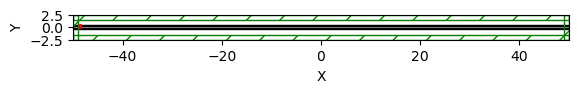
\includegraphics[width=0.8\linewidth]{Figures/wg_design.png}
    \caption{Design of the simulation of a directional coupler. Two parallel symmetric waveguides of width \(w=0.5\ \mu m\) and separated by a gap \(g=0.1\ \mu m\). The guides are made from a material with dielectric constant \(\varepsilon = 12.25\). The simulation is done at resolution \(r=10\) in a simulation space with PML of thickness \(1\ \mu m\).}
    \label{fig:wg_design}
\end{figure}

The directional coupler allows to exchange field from one waveguide to another thanks to the evanescence field. If the two waveguides are identical there is a total exchange of field from one to the other and this happens at the coupling length $\ell_C$. In Fig. \ref{fig:wg_field_fit} is reported the amplitude of the electric field oscillations inside the two guides. The envelope of the field shows how the field is exchanged from one guide to the other.

To evaluate the coupling length two methods were tested. At first, the coupling length was evaluated by finding the minima of the envelope and computing half of their distance. This method isn't very robust and returns wrong results on limit cases.

A second possibility is to evaluate the FFT of the envelope and extract from it a guess on the frequency of the amplitude variation. Using this guess fit the envelope with the function in Eq. \ref{eq:field_fit}
\begin{equation} \label{eq:field_fit}
    f(x) = A \cdot \sin^2{(\omega t + \phi)}
\end{equation}
where \(A\) is the amplitude, \(\omega\) the angular frequency and \(\phi\) the phase.

The result of the fit is reported in Fig. \ref{fig:wg_field_fit}. The fit is done on the electric field in the upper waveguide and it is reported with a $\pi / 2$ shift on the lower waveguide field. From the image, it's clear that the field in the two guides has the same frequency and amplitude while the only difference is the phase.

\begin{figure}[H]
    \centering
    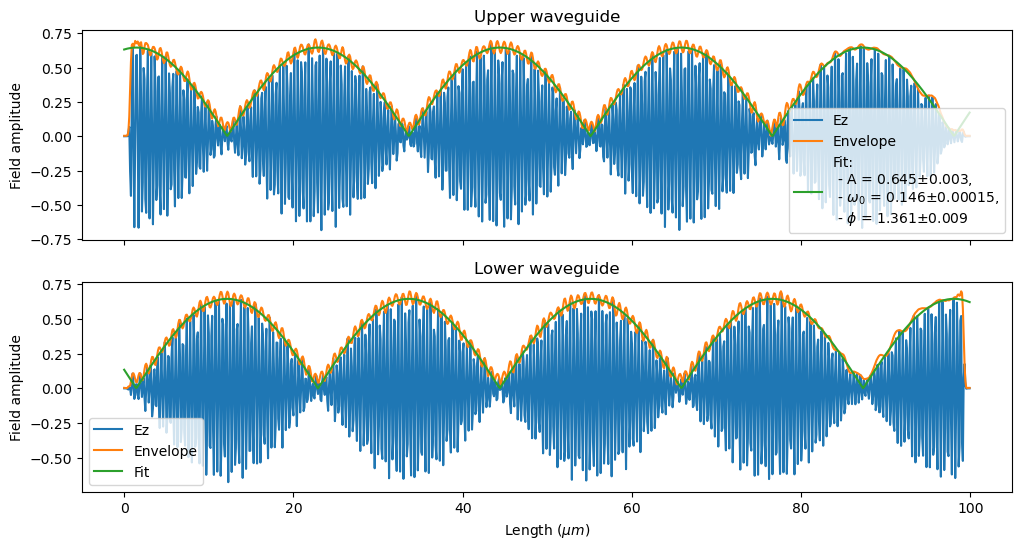
\includegraphics[width=0.6\linewidth]{Figures/wg_field_fit.png}
    \caption{Electric field oscillating along the $z$ axis inside the waveguide and its envelope. The envelope is fitted with the function in Eq. \ref{eq:field_fit}.}
    \label{fig:wg_field_fit}
\end{figure}

\subsection{Symmetric directional coupler}

The difference between a symmetric and asymmetric directional coupler is the amount of transferred energy from one guide to the other. In the symmetric coupler all the field is transferred from one guide to the other while for the asymmetric one only a part of the field is transferred. 

\begin{figure}[H]
    % \centering
    % \begin{subfigure}[b]{0.45\linewidth}
        \centering
        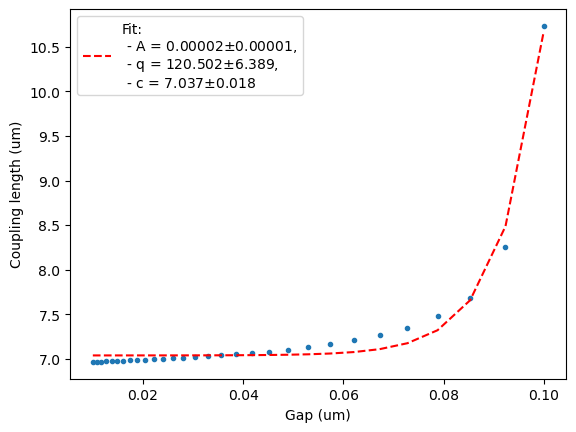
\includegraphics[width=0.5\linewidth]{Figures/wg_coupling_vs_gap.png}
        \caption{Repeated simulation at different values of \(g\) ranging from \(0.01\ \mu m\) to \(0.1\ \mu m\). The dependence of the coupling length on the gap is fitted with the function \(f(x) = A \cdot e^{qg} + c\) as suggested by Eq. \ref{eq:coupling_dependence}.}
        \label{fig:wg_coupling_vs_gap}
        % \end{subfigure}
        % \hfill
        % \begin{subfigure}[b]{0.45\linewidth}
            %     \centering
            %     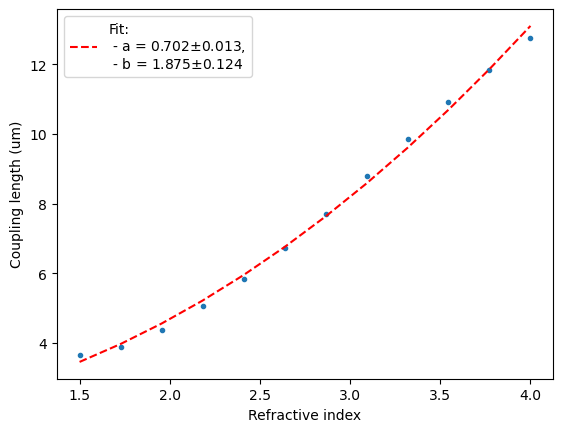
\includegraphics[width=\linewidth]{Figures/wg_coupling_vs_index.png}
            %     \caption{}
            %     \label{fig:wg_coupling_vs_index}
            % \end{subfigure}
\end{figure}
        
The coupling length is defined as $\ell_C = \pi / 2\alpha$ where $\alpha$ is the coupling constant between the guides. For the symmetric coupler the coupling constant depends on several parameters\cite{photonics_book}, among which are the width of the waveguides, the gap between them and the refractive index contrast between the guiding material and the substrate. A more precise dependence from the gap is reported in Eq. \ref{eq:coupling_dependence}
\begin{equation} \label{eq:coupling_dependence}
    \alpha \propto e^{-q\cdot g} 
\end{equation}
where \(g\) is the gap width and \(q\) depends on the effective wavevector, the substrate refractive index and the frequency of the field\cite{photonics_book}.

The simulation was repeated for different values of the gap and the coupling length was extracted with the FFT. The data produced are reported in Fig. \ref{fig:wg_coupling_vs_gap} together with an exponential fit. The agreement with the fit is quite good but it shows that a linear dependence is missing on the base of the exponential.
        
\subsection{Asymmetric directional coupler}

For an asymmetric directional coupler, not all the power is transferred from one guide to the other as can be seen in Fig. \ref{fig:wg_field_asymm}.

\begin{figure}[H]
    \centering
    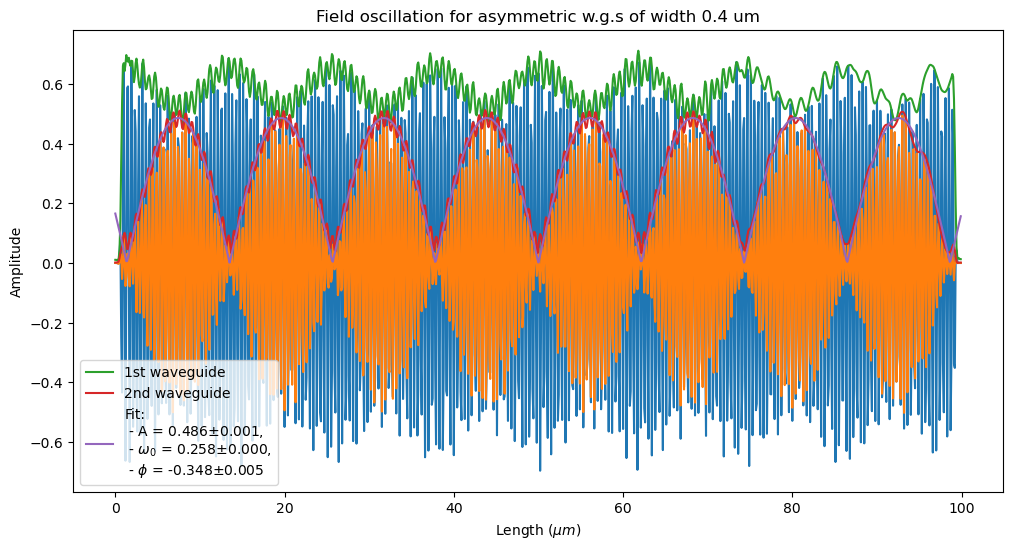
\includegraphics[width=0.8\linewidth]{Figures/wg_field_asymm.png}
    \caption{Electric fields oscillating along the z-axis inside the asymmetric waveguides and their envelopes. The fields were produced by the coupling of two straight waveguides the first one (top waveguide) of width \(0.5\ \mu m\) while the second one (bottom waveguide) of width \(0.4\ \mu m\). The envelope of the field in the bottom waveguide is fitted with the function in Eq. \ref{eq:field_fit} to obtain the coupling length.}
    \label{fig:wg_field_asymm}
\end{figure}

The coupling length can be influenced also by this asymmetry, so the simulation was repeated by changing just the width of the bottom waveguide and the result is represented in Fig. \ref{fig:wg_coupling_vs_asymm}, showing a clear dependence of the coupling length from the asymmetry. The last point in Fig. \ref{fig:wg_coupling_vs_asymm} corresponds to the symmetric coupling.

But another important quantity to consider in case of asymmetry is the power transfer, namely how much of the power in the first guide is transferred to the second guide. The power is computed as the square amplitude of the field in the bottom guide and then normalized for the maximum power in the top guide to obtain the ratio. The ratio changes with the distance from the source, so only the maximum of the ratio is considered and reported in Fig. \ref{fig:wg_power_vs_asymm} as a function of the asymmetry. Again it's clear that the ratio of transferred power depends on the asymmetry in particular the maximum ratio is obtained in the symmetric configuration (last point).

\begin{figure}[H]
    \centering
    \vfill
    \begin{subfigure}[b]{0.48\linewidth}
        \centering
        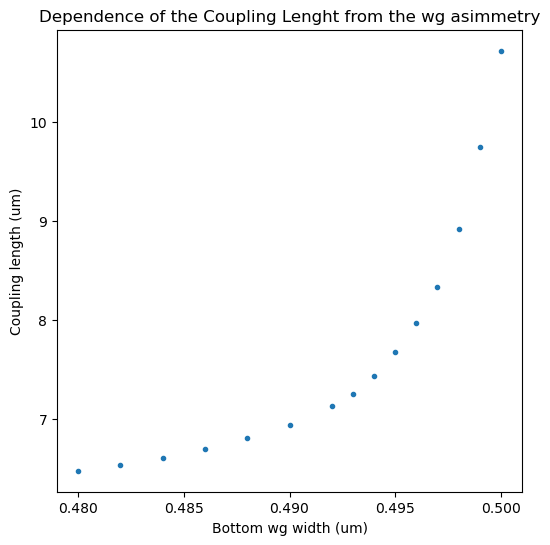
\includegraphics[width=\linewidth]{Figures/wg_coupling_vs_asymm.png}
        \caption{Dependence of the coupling length on the width asymmetry.}
        \label{fig:wg_coupling_vs_asymm}
    \end{subfigure}
    \hfill
    \begin{subfigure}[b]{0.48\linewidth}
        \centering
        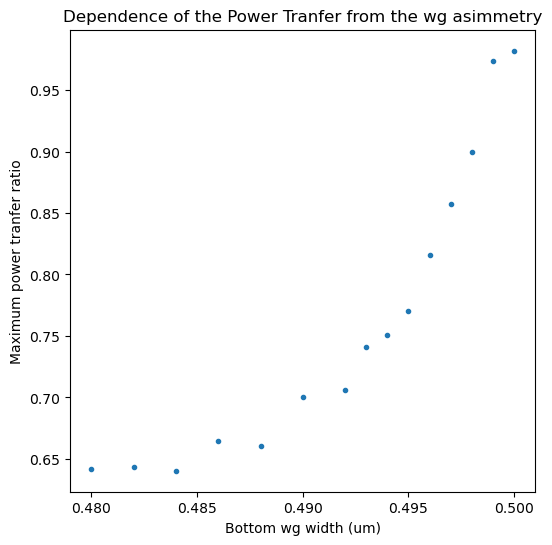
\includegraphics[width=\linewidth]{Figures/wg_power_vs_asymm.png}
        \caption{Dependence of the maximum power transfer ratio on the width asymmetry.}
        \label{fig:wg_power_vs_asymm}
    \end{subfigure}
    \caption{Simulations repeated at different widths of the bottom waveguide ranging from \(0.48\ \mu m\) to \(0.5\ \mu m\). For each simulation, the coupling length and the maximum power transfer ratio are evaluated to show their dependence on the width asymmetry.}
\end{figure}

\section{Bragg reflector}
A distributed Bragg reflector (DBR) is composed of alternating layers of two materials, respectively with refractive index \(n_1 = 1.5\) (silica) and \(n_2 = 2.5\) (titanium dioxide), as represented in Fig. \ref{fig:bragg_design}. This object behaves as a mirror for a certain range of frequency determined by the widths of the layers, the refractive index of the two materials and the number of layers.

\begin{figure}[H]
    \centering
    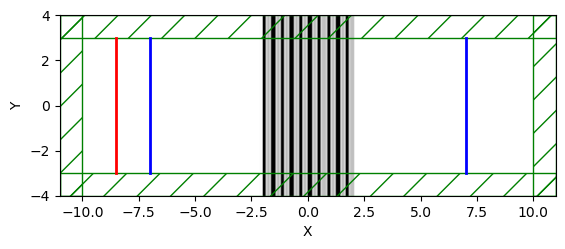
\includegraphics[width=0.8\linewidth]{Figures/bragg_design.png}
    \caption{Design of the simulation of a Bragg reflector. Structure composed of \(N=10\) layers and their widths are computed from Eq. \ref{eq:grating_period}. The simulation is done at resolution \(r=16\) and PML of thickness \(1\ \mu m\).}
    \label{fig:bragg_design}
\end{figure}

To measure the spectrum of this object, two detectors (blue lines in Fig. \ref{fig:bragg_design}) are used, one for the transmitted spectrum and one for the reflected one. The Bragg reflector is shined with a Gaussian source (red line in Fig. \ref{fig:bragg_design}) at wavelength \(\lambda = 1.55\ \mu m\) and frequency width half of the central frequency. The reflector is designed to have this wavelength as the center of its spectrum and this is obtained by imposing the condition of constructive interference in the reflection. This corresponds to constructing the layers following Eq. \ref{eq:grating_period}  
\begin{equation}\label{eq:grating_period}
    n_1 L_1 = \frac{\lambda}{4} \qquad\qquad\qquad n_2 L_2 = \frac{\lambda}{4}
\end{equation}

The reflectance and transmittance spectrum are reported in Fig. \ref{fig:bragg_spectrum}, which shows a very low transmittance in a range of frequencies, paired with a high reflectance in the same range. Considering the transmitted spectrum this range of frequencies is a stop band and its borders are defined as the first maxima of the transmittance.

\begin{figure}[H]
    \centering
    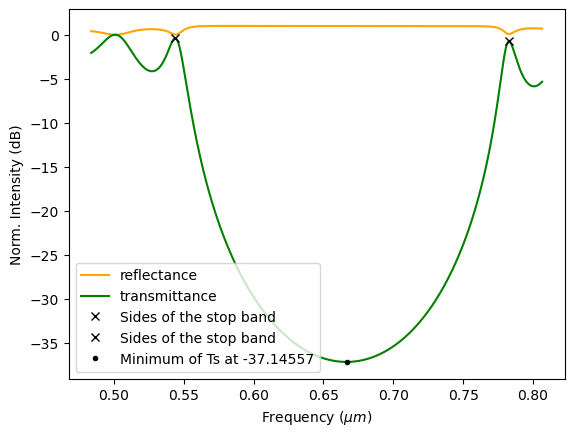
\includegraphics[width=0.6\linewidth]{Figures/bragg_spectrum.png}
    \caption{Transmission and reflection spectra of the DBR shined with a Gaussian source. The reflectivity and transmissivity are reported in dB to highlight how low is the transmittivity in the characteristic range of the Bragg reflector.}
    \label{fig:bragg_spectrum}
\end{figure}

The attenuation in the transmission depends on the refractive index contrast between the two materials and the number of layers as described by Eq. \ref{eq:attenuation}
\begin{equation} \label{eq:attenuation}
    T(\omega_0) \approx 4 \left(\frac{n_1}{n_2}\right)^{2N} 
\end{equation}
The result of the simulation is represented in Fig. \ref{fig:bragg_attenuation_vs_index} and it shows a good agreement with the fit, returning as a parameter the number of layers, compatible with the number set for the simulation, namely \(N=10\).

\begin{figure}[H]
    \centering
    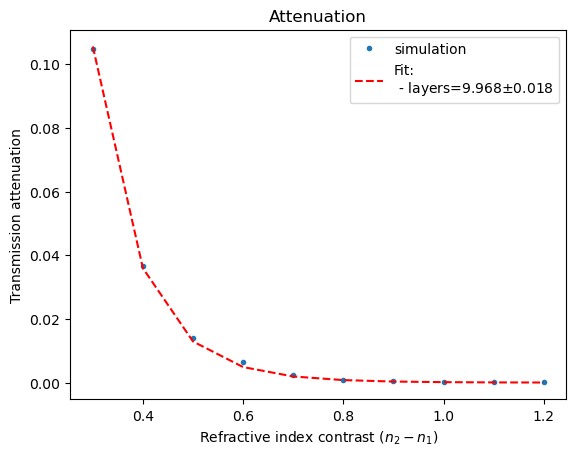
\includegraphics[width=0.6\linewidth]{Figures/bragg_attenuation_vs_index.png}
    \caption{Attenuation of the transmissivity as a function of the refractive indexes contrast. The simulation results are fitted with function in Eq. \ref{eq:attenuation} using as a free parameter the number of layers.}
    \label{fig:bragg_attenuation_vs_index}
\end{figure}

\subsection{Cavity implemented with two DBR}
Mirrors made from DBRs reach a reflectance way higher than even the better metallic mirrors. They are the ideal mirrors for implementing a Fabry-Perot-like cavity, as the one represented in Fig. \ref{fig:bragg_cavity_design}.

\begin{figure}[H]
    \centering
    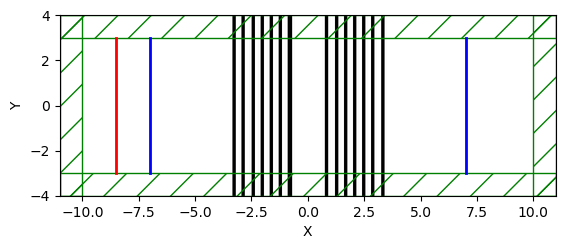
\includegraphics[width=0.8\linewidth]{Figures/bragg_cavity_design.png}
    \caption{Design of a Fabry-Perot cavity using DBRs instead of metallic mirrors. Each mirror is made of 7 layers and differently from the first simulation, the whole simulation space is made from a material of refractive index \(n_2 = 1.5\). The cavity is made from the material with a lower refractive index and it is \(1.5\ \mu m\) wide.}
    \label{fig:bragg_cavity_design}
\end{figure}

The presence of the cavity introduces a resonance in the system resulting in a different spectrum, with a peak in transmission in correspondence with this resonance, as shown in Fig. \ref{fig:bragg_vs_cavity_spectrum}. From this peak in the spectrum, it's possible to extract the Q-factor of the cavity, via a Lorentzian fit around the peak. The result of the fit is shown in Fig. \ref{fig:bragg_cavity_spectrum_fit} and returns a Q-factor\(=52\).

\begin{figure}[H]
    \centering
    \begin{subfigure}[b]{0.45\linewidth}
        \centering
        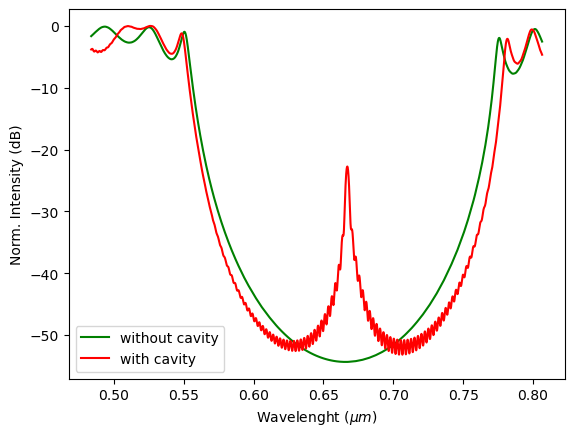
\includegraphics[width=\linewidth]{Figures/bragg_vs_cavity_spectrum.png}
        \caption{Comparison of the transmission spectrum of a Bragg reflector made of 14 layers and the transmission spectrum of a Fabry Perot cavity which uses Bragg reflectors, made of 7 layers, as mirrors.}
        \label{fig:bragg_vs_cavity_spectrum}
    \end{subfigure}
    \hfill
    \begin{subfigure}[b]{0.45\linewidth}
        \centering
        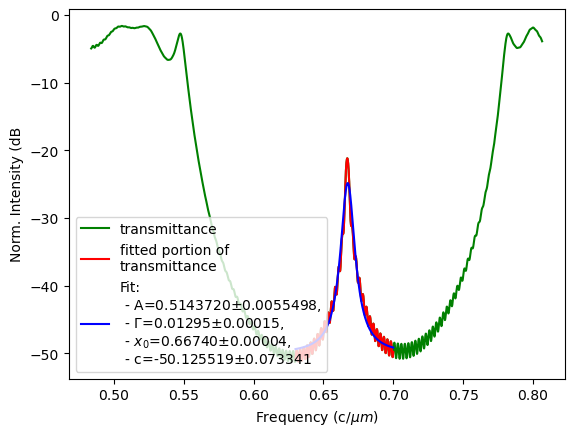
\includegraphics[width=\linewidth]{Figures/bragg_cavity_spectrum_fit.png}
        \caption{Lorentzian fit of the portion of the transmission spectrum of the cavity around the cavity's resonance to extract the Q-factor of the cavity.}
        \label{fig:bragg_cavity_spectrum_fit}
    \end{subfigure}
    \caption{Spectra of the Fabry-Perot cavity constructed using DBRs.}
\end{figure}

The Q-factor depends on the quality of the mirrors, namely from the refractive index contrast between the layers, as shown in Fig. \ref{fig:bragg_cavity_qfactor_vs_index}, in fact, the quality factor of the cavity grows with the contrast, and so with the reflectivity of the mirrors.

\begin{figure}[H]
    \centering
    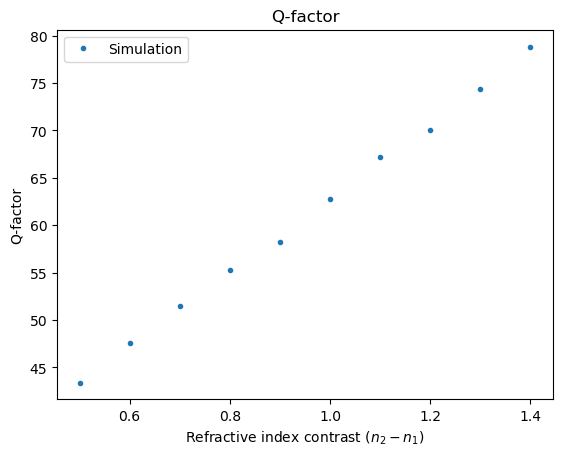
\includegraphics[width=0.6\linewidth]{Figures/bragg_cavity_qfactor_vs_index.png}
    \caption{Dependence of the Q-factor of the cavity from the refractive index contrast.}
    \label{fig:bragg_cavity_qfactor_vs_index}
\end{figure}

\section{Micro Ring Resonator}
A microring resonator is a waveguide closing on itself in a loop. This structure alone is isolated and it requires an additional straight waveguide at a distance \(g\) from the ring to couple light into it, as represented in Fig. \ref{fig:ring_design}. This is called all-pass configuration.

\begin{figure}[H]
    \centering
    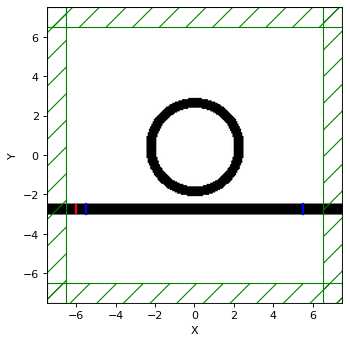
\includegraphics[width=0.6\linewidth]{Figures/ring_design.png}
    \caption{Design of the simulation of a microring resonator. The structure is composed of a ring and a waveguide both with refractive index \(n=1.7\). The waveguide and the ring have width \(w=0.5\ \mu m\) while the ring has an internal radius of \(r=2\ \mu m\). The gap between the guide and the ring is \(g=0.4\ \mu m\). All the simulations are done with a resolution \(r=16\) and PML of thickness \(1\ \mu m\).}
    \label{fig:ring_design}
\end{figure}

A Gaussian source (red line) is put inside the waveguide and then the field oscillating in the waveguide couples to the ring. Inside the ring, the field can be under the condition of constructive interference, namely the resonance condition of the structure.

The source is set to a wavelength equal to a multiple of the perimeter of the ring times the refractive index of the guiding material and its width is about the FSR of the ring. This wavelength is chosen because it's very similar to the resonance frequency except for the refractive index which should be the effective index of the guiding material, as shown by the resonance condition in Eq. \ref{eq:resonance_condition}
\begin{equation}
    m\lambda =  n_{eff} 2\pi r
    \label{eq:resonance_condition}
\end{equation}
where \(n_{eff}\) is the effective refractive index and \(m\) is an integer. 

The resulting transmission and reflection spectrum is shown in Fig. \ref{fig:ring_spectrum}. To find the resonance there are two possible methods: either find the minimum of the spectrum or use the Harminv algorithm (already implemented in MEEP) to find the resonance. The second method returns a resonance at \(\nu = 0.70\ c/\mu m\).

\begin{figure}[H]
    \centering
    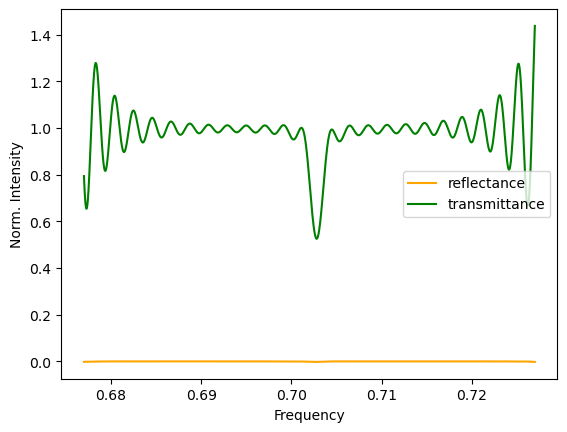
\includegraphics[width=0.8\linewidth]{Figures/ring_spectrum.png}
    \caption{Transmission and reflection spectra of the micro ring resonator coupled to a straight waveguide. The reflectivity is negligible, while transmittivity shows a resonance.}
    \label{fig:ring_spectrum}
\end{figure}

Switching to a continuous source and extracting the field's oscillations in the waveguide, it's possible to compute the phase difference between the field before and after the coupling with the ring. This is done by fitting the field in the two portions of the waveguide using sine functions as shown in Fig. \ref{fig:ring_phase_delay} and then subtracting the phases resulting from the fits.

\begin{figure}[H]
    \centering
    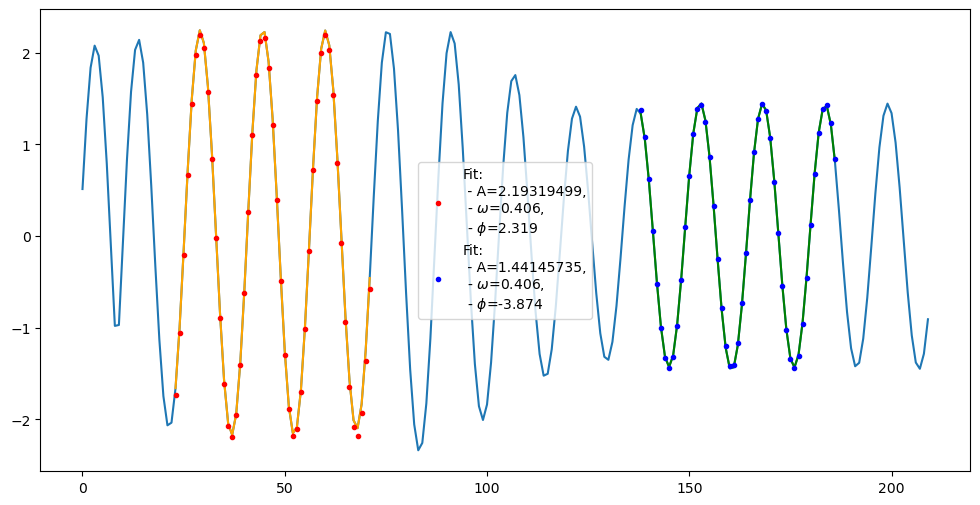
\includegraphics[width=0.8\linewidth]{Figures/ring_phase_delay.png}
    \caption{Electric field oscillating along the z-axis inside the waveguide. To obtain the phase difference produced by the coupling with the ring, two portions of the field are selected (orange and green portions) to be fitted and extract the phase difference between the field before and after the ring. The parameters resulting from the fit are reported in the legend, where the red dots represent the fit before the ring and the blue dots the fit after.}
    \label{fig:ring_phase_delay}
\end{figure}

In order to have a more precise transmission spectrum, the simulations are repeated with continuous sources at different frequencies. The spectrum is then fitted with a Lorentzian function to obtain the Q-factor of the ring resonator which is \(Q=365.5\). The resonance found here corresponds to the one computed from the Harminv algorithm.

\begin{figure}[H]
    \centering
    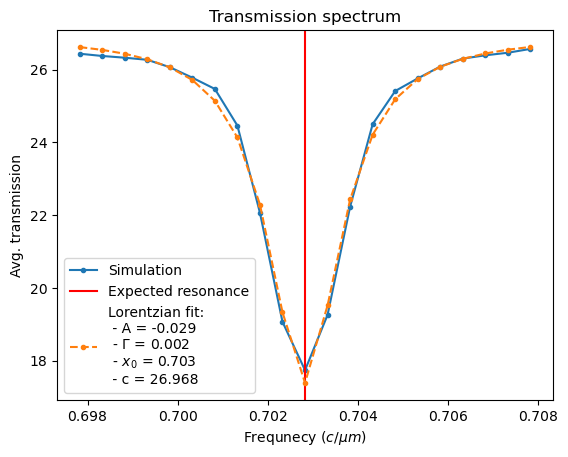
\includegraphics[width=0.7\linewidth]{Figures/ring_frequency_sweep.png}
    \caption{Transmission spectrum of the structure centered around the resonance and obtained by a sweep in the frequency of a continuous source.}
    \label{fig:ring_frequency_sweep}
\end{figure}

Another important behavior of the ring resonator is the change of phase difference in the three coupling regimes, namely the fields are in phase (\(\Delta \phi = 0\)) in under coupling, and they are in antiphase (\(\Delta \phi = \pi\)) in over coupling while they have a \(\Delta \phi = \frac{\pi}{2}\) phase difference in critical coupling.

The different coupling regimes depend on the gap between the ring and the straight waveguide. Repeating the simulations for values of the gap ranging from \(0.08\ \mu m\) to \(0.35\ \mu m\), the changes in phase difference are reported in Fig. \ref{fig:ring_phase_vs_gap}. 

The graph shows the over-coupling behavior for low values of the gap and the under-coupling behavior for the high values of the gap.

\begin{figure}[H]
    \centering
    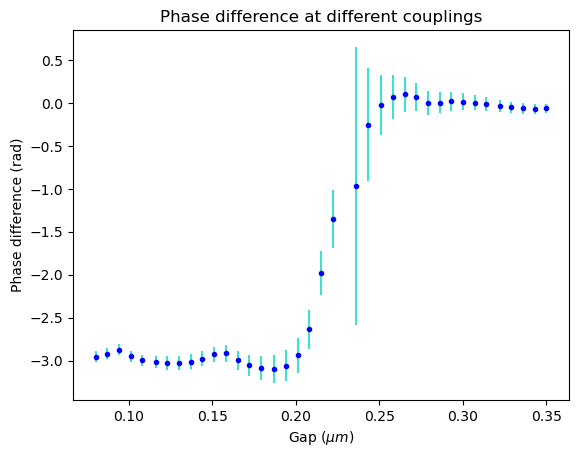
\includegraphics[width=0.7\linewidth]{Figures/ring_phase_vs_gap.png}
    \caption{Variation of the phase difference for a variation of the gap between the ring and the guide. The phase difference is obtained from the electric field fits, as described above.}
    \label{fig:ring_phase_vs_gap}
\end{figure}

\printbibliography
% \addcontentsline{toc}{chapter}{Bibliography}
\end{document}
